
\section{\ix Implementation}
\label{sec:impl}

\begin{table*}[t]
\centering
\begin{small}
\begin{tabular}{|l|l|l|}
\hline
\multicolumn{3}{|c|}{{\bf System Calls (batched)}} \\
\hline
connect &             cookie, dst\_IP, dst\_port		& Opens a connection\\
accept &              handle, cookie				& Accepts a connection\\
sendv &               handle, scatter\_gather\_array		& Transmits a scatter-gather array of data\\
recv\_done &          handle, bytes\_acked			& Advances the receive window and frees memory buffers\\
close &               handle					& Closes or rejects a connection\\
\hline  \hline
\multicolumn{3}{|c|}{{\bf Event Conditions}} \\
\hline
{\bf Type} &           {\bf Parameters}  &
{\bf Description}\\
knock  &               handle, src\_IP, src\_port		& A remotely initiated connection was opened \\
connected &            cookie, outcome				& A locally initiated connection finished opening \\
recv &                 cookie, mbuf\_ptr, mbuf\_len		& A message buffer was received \\
sent &                 cookie, bytes\_sent, window\_size	& A send completed and/or the window size changed \\
dead &                 cookie, reason				& A connection was terminated \\
\hline
\end{tabular}
\caption{\ix system calls and event conditions API. 
}
\label{tbl:api}
\end{small}
\end{table*}



We now describe the \ix prototype.  The current implementation uses
the VT-x featurs available on all x86-64
severs~\cite{DBLP:journals/computer/UhligNRSMABKLS05}. However, it can
be ported to any architecture with virtualization support, such as ARM
and Power.

% We start
% with an overview of the \ix kernel (\S\ref{sec:impl:kernel}), describe
% the environment surrounding \ix (\S\ref{sec:impl:env}), and how \ix is
% implemented as a coherency-free kernel (\S\ref{sec:impl:cohfree}).


%the benefits of having \ix run as a guest
%operating system (\S\ref{sec:impl:guest}), its native API at the
%kernel/user boundary (\S\ref{sec:impl:api}), the implementation of the
%networking stack (\S\ref{sec:impl:stack}), the implications on
%congestion management and flow control (\S\ref{sec:impl:net}), the
%benefits and consequences of coherence-free execution
%(\S\ref{sec:impl:cohfree}), and finally our approach to compatibility
%(\S\ref{sec:impl:libix}).

\subsection{Overview}
\label{sec:impl:overview}

Fig.~\ref{fig:cp-dp} presents the \ix architecture, including the
control plane, a number of dataplanes, and applications. The hardware
environment includes one or more multi-queue NICs with RSS support and
a multi-core server.

The \ix control plane consists of the full Linux kernel and
\texttt{IXCP}, a user-level program. The Linux kernel initializes PCIe
devices, such as the NICs, and provides the basic mechanisms for
resource allocation to the dataplanes, including cores, memory, and
network queues. Equally important, Linux provides the wide range of
system calls and services necessary for compatibility with a wide
range of applications, such as file system and signals
support. \texttt{IXCP} monitors resource usage and dataplane
performance and implements resource allocation policies. The
development of efficient allocation policies involves understanding
difficult tradeoffs between dataplane performance, energy
proportionality, and resource sharing between co-located applications
as their load varies over time. We leave the design of such policies
to future work and focus this paper on the \ix dataplane architecture.

We run the Linux kernel in VMX root ring 0, the mode typically used to
run the hypervisor in virtualized
systems~\cite{DBLP:journals/computer/UhligNRSMABKLS05}. We use the
Dune system within Linux to enable dataplanes to run as library-based
OS in the VMX non-root ring 0, the mode typically used to run guest
OSes in virtualized systems~\cite{belay2012dune}. The applications run
in ring 3 as usual. This approach provides dataplanes with direct
access to hardware functions such as page tables and provides full
protection between the control plane, dataplanes, and untrusted user
code. \christos{do we need more details for people that don't know
  dune? should we explicitly say that most web-scale apps are deployed
  without VMs so taking over VMX is not a problem?}

% \myparagraph{Separation and protection of control and data plane:}
% Each \ix instance and its applications runs as a distinct Dune process
% while control plane functions, including the control and monitoring of
% dataplane, is performed by scripts and daemons of the host
% environments.  This provides protection between control and
% dataplanes. Within each dataplane, \ix further protects itself from
% the untrusted application through virtual memory and by running it at
% userlevel.

% Section Move to the discussion session or future work
% \myparagraph{Elasticity policies:} In contrast to the mechanisms,
% which are generic, different policies can be envisioned to meet
% different use cases and optimization functions.  If neither energy
% proportionality or server consolidation is of any concern, the control
% plane can obviously launch a single dataplane instance configured with
% the maximal available physical resources.  In more realistic
% scenarios, the dataplane is ``right-sized'' to meet its service-level
% agreements with minimal resource allocations.  The control plane can
% further dynamically add or revoke CPUs from a dataplane instances,
% e.g., when the dataplane signals some sustained congestion or
% violation of its service-level agreements, or conversely when the
% allocated CPU resources are underutilized.


Each \ix dataplane supports a single, multithreaded POSIX
application. For instance, Fig.~\ref{fig:cp-dp} shows one dataplane
for a multi-threaded \texttt{memcached} server and another dataplane
for a multi-threaded \texttt{ngix} server. The control plane allocates
resources to each dataplane in a coarse-grain manner. Core allocation
is controlled through real-time priorities and and \texttt{cpumasks};
memory is allocated in 2MB and 1GB chunks; each NIC hardware queue is
assigned to a single dataplane. This approach avoids the overheads and
unpredictability of fine-grain time multiplexing of resources between
demanding applications~\cite{Leverich:RHSU:2014}.

The \ix dataplane operates as a single address-space OS and supports
two distinct thread types within the shared, user-level address space:
(i) \emph{elastic threads} which interact with the \ix dataplane to
initiate and consume network I/O and (ii) \emph{background threads}
Both elastic and background threads can issue arbitrary POSIX system
calls that are are merely intermediated by the dataplane and handled
by the Linux kernel.  Elastic threads are expected to \emph{not} issue
blocking calls because of the adverse impact on network behavior and
performance. Similarly, each elastic thread makes exclusive use of a
core or hyperthread allocated to the dataplane in order to achieve
high performance with predictable latency. In contrast, multiple
background threads may timeshare an allocated hyperthread. Hence, an
application like \texttt{memcached} allocated four hyperthreads may
use four elastic threads to serve external requests or temporarily
transition to three elastic threads when some background threads need
to execute tasks such as garbage collection. When the control plane
revokes or allocates an additional hyperthread using a protocol
similar to the one used in Exokernel~\cite{DBLP:conf/sosp/EnglerKO95},
the dataplane must adjust the number of elastic threads it uses.

% We extended the Dune sandboxing mechanisms to support the initial load
% of multi-threaded applications into the userlevel address space, to
% launch both elastic and background threads.

\subsection{Dataplane API and Operation}
\label{sec:impl:kernel}

Elastic threads interact with the \ix dataplane through three
asynchronous, non-blocking mechanisms summarized in
Table~\ref{tbl:api}: they can issue \emph{batched systems calls} to
the dataplane; they consume \emph{event conditions} generated by the
dataplane; and they have direct, but safe, access to message buffers
(\emph{mbuf}) containing incoming networking payload. The latter is
quite different from traditional POSIX sockets and allows for
zero-copy access to network incoming traffic.  The application can
then hold on to these message buffers and release them via a batched
system call.  \ix also differs in directly exposing flow control
conditions to application. The \texttt{sendv} batched system call does
not synchronously return the number of bytes sent. Instead, the
\texttt{Recv} event condition provides that information at a later point

In addition to the native API in Table~\ref{tbl:api}, we also
developed a user-level library that exposes a near identical API to
\texttt{libevent}. This library simplifies provides compatibility for
legacy applications and significantly simplifies the development of
new applications. \christos{add one sentence on what is different
  here, since we mention ``near}

\begin{figure}
%\hspace*{-0.25in}\centering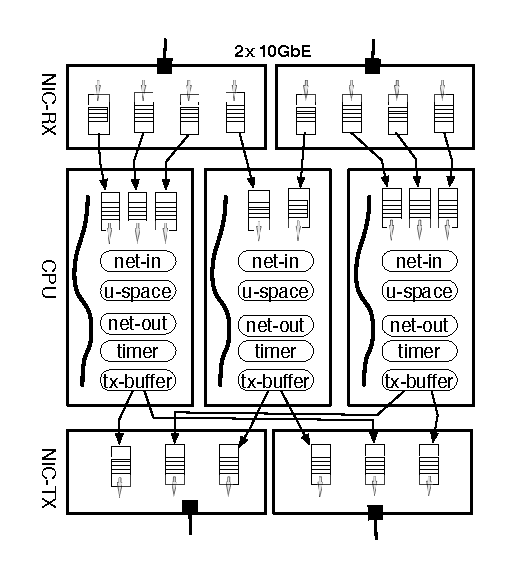
\includegraphics{figs/queues-cores.eps}
\centering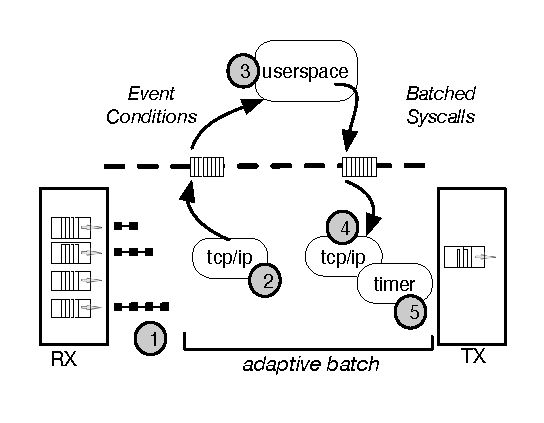
\includegraphics{figs/pipeline}
\caption{The IX pipeline.}
\label{fig:queues-cores}
\end{figure}

 

Fig.~\ref{fig:queues-cores} illustrates the run-to-completion
operation of elastic threads in the \ix dataplane. Each elastic thread
is associated with a specific set of receive queues from one or more
NICs. Each NIC uses RSS to implement flow-consistent hashing and
distribute incoming packets to queues. The queues are mapped in the
server's main memory and the NIC is given a set of buffer descriptors
that allow it to transfer incoming packets to memory using DMA.  The
elastic thread (1) polls the receive queues it is responsible for and
potentially posts fresh buffer descriptors to the NIC for use with
future incoming packets. The elastic thread (2) processes a bounded
number of packets through the TCP/IP networking stack, thereby
generating event conditions. Next, the elastic thread (3) passes
control to the user-space applications, which consumes all event
conditions. Assuming that the incoming packets include remote
requests, the application processes these requests and responds with a
batch of system calls. Upon return of control from user-space, \ix (4)
processes all system calls, and in particular the ones that direct
outgoing TCP/IP traffic. It also (5) runs all kernel timers in order
to ensure compliant TCP behavior and (6) places outgoing Ethernet
frames in the NIC's descriptor rings for transmission. \christos{don't
  we also need to ring a doorbell to initiate the outgoing DMA?}

The \ix dataplane consists of 37 KSLOC. We leveraged existing
codebases in its development: 43\% is derived from the Intel NIC
device driver~\cite{ref?}, 23\% from the lwIP TCP/IP
stack~\cite{dunkels2001design}, and 16\% from the Dune library.  All
three code bases are highly modified for \ix. The rest is
approximately 7 KSLOC of new code. We chose lwIP as a starting point
for TCP/IP processing because of its modularity and is maturity as a
compliant, feature-rich networking stack. It allows us to be
RFC-compliant for TCP, UDP, ARP, ICMP and LACP. Since lwIP was
optimized for memory efficiency in embedded environments, we had to
radically change its internal data structures for multi-core
scalability and fine-grain timer management. We did not yet optimize
the lwIP code for performance. Hence, there is room for improvement in
the results shown in \S\ref{sec:eval}. 


\subsection{Multi-core Scalability}
\label{sec:impl:cohfree}

The \ix dataplane is optimized for multi-core scalability as elastic
threads operate in a synchronization and coherence free manner in the
common case. This is a stronger requirement than lock-free
synchronization, which requires expensive atomic instructions even
when a single thread uses a particular lock in the common
case~\cite{DBLP:conf/sosp/DavidGT13}.  This was made possible 
through a set of conscious design and implementation tradeoffs. 

First, the \ix API is commutative. Events are processed independently
on each elastic thread. Cookies identify flows but cannot be exchanged
between elastic threads. There is no file descriptor namespace.
According to the commutativity rule, system call implementations can
only be coherence-free if the API itself is
commutative~\cite{DBLP:conf/sosp/ClementsKZMK13}.

Second, the API implementation is carefully optimized.  Each elastic
thread manages its own memory pools, hardware queues, event condition
queue, and batched system call queue. No synchronization is required
to access any of them. The implementation of event conditions and
batched system calls benefits directly from the explicit, cooperative
control flow transfers between \ix and the application by the elastic
thread.  Since there is no concurrent execution by producer and
consumer, event conditions and batched system calls are implemented as
arrays without relying on lock-free synchronization primitives based
on atomics.

Third, the use of flow-consistent hashing at the NICs ensures that
each elastic thread operates on a disjoint subset of incoming TCP
flows. Hence, no synchronization or coherence occurs during the
processing of incoming packets for a server application. For client
application with outbound connections, the solution is more complex.
\christos{The following needs some cleanup/simplification} For
outbound connections, \ix selects the source ephemeral port based on
the requesting elastic thread. Since the Toeplitz hash function cannot
be reversed, \ix simply probes the ephemeral range and computes the
Toepliz hash until a match is found.  Consequently, communication
between an \ix client and a server may required up to one flow per
elastic thread.  As a side effect of the implementation, ephemeral
source port no longer form namespaces, which allows an \ix client to
support millions of outgoing connections.

\ix does have a small number of shared structures, including some that
require synchronization on updates.  For example, the ARP table is
shared by all elastic threads and is protected by RCU
locks~\cite{mckenney1998read}, Hence, the common case reads are
coherency-free but the rare updates are not. \ix also requires
synchronization when the control plane reallocates resources between
dataplanes.  For instance, when a core is revoked from a dataplane,
the corresponding incoming queues must be assigned to another elastic
thread. Such events are rare because resource allocation happens in a
coarse-grain manner. Finally, the application code may include
inter-thread communication and synchronization. While using \ix does
not eliminate the need to develop scalable application code, it
ensures that there are no scaling bottlenecks in the system and
protocol processing code. 

\subsection{Cooperative Flow Control}
\label{sec:impl:cohfree}

\christos{we need a short section here that goes over cooperative flow
  control and why it is cool long term (including the zero copy
  discussion). I think a a subset of the following paragraph fits here too}

\myparagraph{Security model:} Applications are
untrusted and can not access kernel memory (except for message
buffers) or network hardware.  No sequence of batched system calls or
other user-level actions can be used to violate correct adherence to
TCP and other network specifications.  Furthermore, the dataplane can
be used to enforce network security policies (e.g., iptables or Amazon
Security Groups) or to implement the network virtualization functions
typically done in a hypervisor~\cite{nsdi:nsx}.  However, and as a
consequence of the zero-copy model, applications have read-only access
to entire message buffers, including protocol headers.  Flow control
and receive buffer management is, however, entrusted to the user
runtime. Applications could misuse this ability to use up all of their
available memory, but it would only harm its own \ix instance.


